\section{Direction Estimation}
\label{sec:03_direction}

After the \lstinline!WhistleData! was filled by the \lstinline!WhistleDetection!,
the \lstinline!WhistleLocalization! start to process the buffered microphone data.
First, the frames which will be considered for the calculation of the \ac{TDOA}
are chosen.
Different criteria apply for the correlation methods and phase method, but the
resulting \lstinline!start_index! of the signal start detection implementation
\cref{sec:03_signalStartDetection} is utilized in both.
% -------------------------------------------------------------

For the correlation methods in \cref{sec:02_cc} and \cref{sec:02_gcc}, the beginning
of the signal is chosen where the change from noise to signal is visible at best.
\lstinline!frame_size/2! samples before and after the \lstinline!start_index! are defined
as frame.
It gets undecidable which signal came first for later frames. Thus, if the start detection
is inaccurate the resulting \ac{TDOA} is not reliable.
% -------------------------------------------------------------

Regarding the phase method,
%\cref{sec:02_phase}%,
\missing[]{reference to 02 phase}
the frames with the same maximal frequency for each channel are used for the
phase difference calculation.
The phase difference of this frequency is then considered for the phase difference
calculation. %\cref{sec:03_phase}
\missing[]{reference to 03 phase}
% -------------------------------------------------------------

Before determining the delays, the frames are windowed with a Hann window and can be
normalized optionally.
According to the method, the delays between the channels are computed to conclude the
consequential direction candidates.
For each delay between neighboring channels, one positive signed and one negative
signed candidate arise.

% -------------------------------------------------------------
\Cref{lst:03_direction} lists the single steps that are necessary for the sound source
candidates in robot coordinates.
Positive values for delays mean that the signal first arrived at the \lstinline!base_channel!.
Exemplary considering the case where the delay is equal to the positive maximal delay,
the signal was first
detected by the \lstinline!base_channel! before arriving at the \lstinline!next_channel!.
As a consequence, the direction of the source is opposite to the channel vector and equal
to the \lstinline!max_delay_vector!.
Generally, the direction candidates are calculated relative to this \lstinline!max_delay_vector!,
where the angle $\gamma'$ is determined by \cref{eq:02_tdoaAngle}.
\Cref{fig:03_tdoaCode} shows resulting candidates of same situation as \cref{fig:02_tdoa} with
the resulting possible source directions \lstinline!candidates!.
% -------------------------------------------------------------
\code{tdoa}{0}{10}{Calculation of whistle direction in robot coordinates.}{03_direction}
% -------------------------------------------------------------
\begin{figure}[ht]
	\centering
		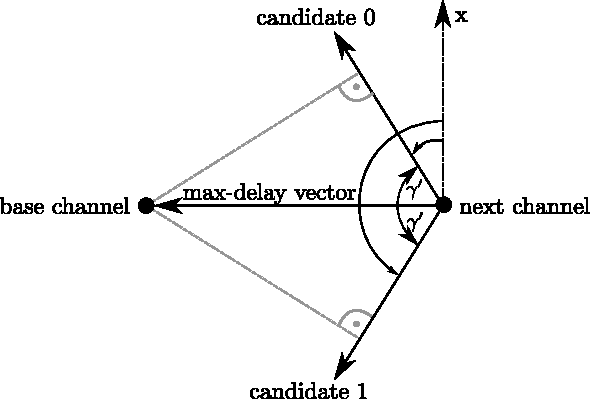
\includegraphics[width=0.6\columnwidth]{figures/tdoa_code}
	\caption{Illustration of the resulting candidates of \ac{TDOA} implementation.}
	\label{fig:03_tdoaCode}
\end{figure}

As there exists the exceptional case that the sidewise and forward delays are both small
as considered in \cref{sec:02_distance}, the invalidity of
\lstinline!small_y_shift && small_x_shift! as notated in \cref{lst:03_distance} must
be confirmed.
If so, not only the direction but also an approximate distance can be determined
as discussed in \cref{sec:03_distance}.
Otherwise, the direction with the smallest difference between the
candidates of each channel is submitted as final result.

A final result of the sound source direction relative to one robot must be defined
a the eight candidates of the four delays.
Therefore, the sum of the difference for each combination of the candidates
is taken as decisive criterion to find a final direction angle $\gamma$ in robot coordinates.
During research, different factors like signal strength were tested to include
more properties of the signal. They will be topic in \ref{sec:04_direction}.